\XtoCBlock{Sin3Gen}
\label{block:Sin3Gen}
\begin{figure}[H]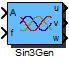
\includegraphics{Sin3Gen}\end{figure} 

\begin{XtoCtabular}{Inports}
A & Amplitude\tabularnewline
\hline
f & Frequency\tabularnewline
\hline
\end{XtoCtabular}


\begin{XtoCtabular}{Outports}
u & Sine wave output phase u\tabularnewline
\hline
v & Sine wave output phase v\tabularnewline
\hline
w & Sine wave output phase w\tabularnewline
\hline
\end{XtoCtabular}

\begin{XtoCMaskParamTabular}{Mask Parameters}
\rowcolor[gray]{0.8}\textbf{Name} & \textbf{ID} & \textbf{Description}\tabularnewline\hline
fmax & 1 & Maximum Frequency in Hz\tabularnewline
\hline
Offset & 2 & Offset\tabularnewline
\hline
ts\_fact & 3 & Multiplication factor of base sampling time (in integer format)\tabularnewline
\hline
\end{XtoCMaskParamTabular}

\subsubsection*{Description:}
Generation of a 3 sine waves with amplitude (A) and frequency (f).

% include optional documentation file
\InputIfFileExists{\XcHomePath/Library/General/Doc/Sin3Gen_Info.tex}{\vspace{1ex}}{}

\subsubsection*{Implementations:}
\begin{tabular}{l l}
\textbf{FiP16} & 16 Bit Fixed Point Implementation\tabularnewline
\textbf{FiP32} & 32 Bit Fixed Point Implementation\tabularnewline
\textbf{Float32} & 32 Bit Floating Point Implementation\tabularnewline
\textbf{Float64} & 64 Bit Floating Point Implementation\tabularnewline
\end{tabular}

\XtoCImplementation{FiP16}
\nopagebreak[0]

16 Bit Fixed Point Implementation

\begin{XtoCtabular}{Inports Data Type}
A & int16\tabularnewline
\hline
f & int16\tabularnewline
\hline
\end{XtoCtabular}

\begin{XtoCtabular}{Outports Data Type}
u & int16\tabularnewline
\hline
v & int16\tabularnewline
\hline
w & int16\tabularnewline
\hline
\end{XtoCtabular}

\ifdefined \AddTestReports
\InputIfFileExists{\XcHomePath/Library/General/Doc/Test-Results/Test_Sin3Gen_FiP16.tex}{}{}
\fi
\XtoCImplementation{FiP32}
\nopagebreak[0]

32 Bit Fixed Point Implementation

\begin{XtoCtabular}{Inports Data Type}
A & int32\tabularnewline
\hline
f & int32\tabularnewline
\hline
\end{XtoCtabular}

\begin{XtoCtabular}{Outports Data Type}
u & int32\tabularnewline
\hline
v & int32\tabularnewline
\hline
w & int32\tabularnewline
\hline
\end{XtoCtabular}

\ifdefined \AddTestReports
\InputIfFileExists{\XcHomePath/Library/General/Doc/Test-Results/Test_Sin3Gen_FiP32.tex}{}{}
\fi
\XtoCImplementation{Float32}
\nopagebreak[0]

32 Bit Floating Point Implementation

\begin{XtoCtabular}{Inports Data Type}
A & float32\tabularnewline
\hline
f & float32\tabularnewline
\hline
\end{XtoCtabular}

\begin{XtoCtabular}{Outports Data Type}
u & float32\tabularnewline
\hline
v & float32\tabularnewline
\hline
w & float32\tabularnewline
\hline
\end{XtoCtabular}

\ifdefined \AddTestReports
\InputIfFileExists{\XcHomePath/Library/General/Doc/Test-Results/Test_Sin3Gen_Float32.tex}{}{}
\fi
\XtoCImplementation{Float64}
\nopagebreak[0]

64 Bit Floating Point Implementation

\begin{XtoCtabular}{Inports Data Type}
A & float64\tabularnewline
\hline
f & float64\tabularnewline
\hline
\end{XtoCtabular}

\begin{XtoCtabular}{Outports Data Type}
u & float64\tabularnewline
\hline
v & float64\tabularnewline
\hline
w & float64\tabularnewline
\hline
\end{XtoCtabular}

\ifdefined \AddTestReports
\InputIfFileExists{\XcHomePath/Library/General/Doc/Test-Results/Test_Sin3Gen_Float64.tex}{}{}
\fi
